%%%%%%%%%%%%%%%%%%%%%%%%%%%%%%%%%%%%%%%%%
% FRI Data Science_report LaTeX Template
% Version 1.0 (28/1/2020)
% 
% Jure Demšar (jure.demsar@fri.uni-lj.si)
%
% Based on MicromouseSymp article template by:
% Mathias Legrand (legrand.mathias@gmail.com) 
% With extensive modifications by:
% Antonio Valente (antonio.luis.valente@gmail.com)
%
% License:
% CC BY-NC-SA 3.0 (http://creativecommons.org/licenses/by-nc-sa/3.0/)
%
%%%%%%%%%%%%%%%%%%%%%%%%%%%%%%%%%%%%%%%%%


%----------------------------------------------------------------------------------------
%	PACKAGES AND OTHER DOCUMENT CONFIGURATIONS
%----------------------------------------------------------------------------------------
\documentclass[fleqn,moreauthors,10pt]{ds_report}
\usepackage[english]{babel}

\graphicspath{{fig/}}




%----------------------------------------------------------------------------------------
%	ARTICLE INFORMATION
%----------------------------------------------------------------------------------------

% Header
\JournalInfo{FRI Natural language processing course 2021}

% Interim or final report
\Archive{Project report} 
%\Archive{Final report} 

% Article title
\PaperTitle{Cross-Lingual Question Generation} 

% Authors (student competitors) and their info
\Authors{Igor Nikolaj Sok, Tian Grumerec, and Jurij Dolenc}

% Advisors
\affiliation{\textit{Advisors: Slavko Žitnik}}

% Keywords
\Keywords{Information retrieval, Natural Language Processing, Keyword3 ...}
\newcommand{\keywordname}{Keywords}


%----------------------------------------------------------------------------------------
%	ABSTRACT
%----------------------------------------------------------------------------------------

\Abstract{
The abstract goes here. The abstract goes here. The abstract goes here. The abstract goes here. The abstract goes here. The abstract goes here. The abstract goes here. The abstract goes here. The abstract goes here. The abstract goes here. The abstract goes here. The abstract goes here. The abstract goes here. The abstract goes here. The abstract goes here. The abstract goes here. The abstract goes here. The abstract goes here. The abstract goes here. The abstract goes here. The abstract goes here. The abstract goes here. The abstract goes here. The abstract goes here. The abstract goes here. The abstract goes here.
}

%----------------------------------------------------------------------------------------

\begin{document}

% Makes all text pages the same height
\flushbottom 

% Print the title and abstract box
\maketitle 

% Removes page numbering from the first page
\thispagestyle{empty} 

%----------------------------------------------------------------------------------------
%	ARTICLE CONTENTS
%----------------------------------------------------------------------------------------

\section*{Introduction}
Natural language processing is currently a very actual and rapidly developing field of computer science. In the sub field of Information Retrieval (IR), there is much ongoing research that aims to improve a language models ability to understand the text and pick up its core meaning. In the scope of our project we aim to develop a model, capable of processing text and understanding it to a point, where it can provide questions based on the text in many languages. To achieve this we plan to expand on the existing Doc2Query approach and include a T5 translation model to enable cross-lingual question generation. We will benchmark our solution using the BEIR\cite{DBLP:journals/corr/abs-2104-08663} benchmark and the benchmark included in the SQuAD\cite{DBLP:journals/corr/RajpurkarZLL16} paper. In addition we will manually check provided question-answer pairs for relevance.

\subsection{Related work}

In the article \textit{Exploring the Limits of Transfer Learning with a Unified Text-to-Text Transformer}\cite{DBLP:journals/corr/abs-1910-10683} the authors discuss a model for streamlining the task of transfer learning. Transfer learning is a procedure that enhances Natural Language Processing (NLP) by pre-training models on data-rich tasks and fine-tuning them on specific downstream tasks. The authors propose a unified framework for converting all text-based language problems into a text-to-text format. In the scope of their study they compared pre-training, unlabelled datasets, different architectures and more on many language understanding tasks and achieved state of the art results on many benchmarks including question answering and summarization. The model that achieved the best results was a T5 encoder-decoder model. They introduced a "Colosal Clean Crawled Corpus" (C4) dataset, which provides enough diverse data for general language understanding, which significantly boosts the models performance.

The authors of the article \textit{Sentence-T5: Scalable Sentence Encoders
from Pre-trained Text-to-Text Models}\cite{ni2021sentencet5} explore sentence embedding for text-to-text NLP applications, focusing on extracting embeddings from T5 models. The authors examine three approaches to generate sentence embeddings from T5 models: using the first token representation of the encoder, averaging all token representations from the encoder and using the first token representation from the decoder. They also introduce a SentGLUE benchmark for sentence representation, which extends SentEval to include nine tasks from the GLUE benchmark, which better compares performance. The authors concluded that that encoder-only mod-
els have strong transfer performance while encoder-
decoder models perform better on textual similarity
tasks.

In the article \textit{Document Expansion by Query Prediction}\cite{DBLP:journals/corr/abs-1904-08375} the authors introduce a model called Doc2Query; a model that for a given document, predicts a query, which can then be appended to the document. The authors trained a sequence-to-sequence model that generates possible questions that the document might answer. This can be used to better index documents, to provide more accurate document search for search engines, help with Domain specific training data generation and can be used for generating pairs for a given collection of unlabelled texts. Doc2Query uses a simple seq-to-seq transformer to produce a query from the document, both of which are segmented using BPE\cite{sennrich2016neural} after being tokenized with the MOSES tokenizer. The document and queries are then truncated to avoid excessive memory usage. Once the model is trained, it predicts 10 queries using the top-k random sampling. The model was trained on the MSMARCO\cite{DBLP:journals/corr/NguyenRSGTMD16} dataset.

The article \textit{Doc2Query--: When Less is More}\cite{gospodinov2023doc2query} expands on the Doc2Query approach by trying to eliminate the "hallucinations" that Doc2Query might produce by generating questions that are not present in the source text. The authors argue that Doc2Query is prone to hallucination and that this harms retrieval effectiveness and inflates the index size. They explore and propose techniques for filtering out these harmful queries prior to indexing. Doc2Query-- estimates the relevance of a query with relevance models. With this the retrieval effectiveness of indexes improves by up to 16\%, while also reducing index size. The major drawback of this approach is the higher computational cost that arises by removing irrelevant queries.

The authors of the article \textit{BEIR: A Heterogeneous Benchmark for Zero-shot Evaluation}\cite{DBLP:journals/corr/abs-2104-08663} propose a new robust heterogeneous evaluation benchmark for IR (Benchmarking-IR, BEIR), leveraging a careful selection of 18 publicly selected datasets from diverse text retrieval tasks and domains. The authors evaluated 10 state of the art IR systems with their BEIR benchmark to find their strengths and weaknesses, where it proved to be a good benchmark for IR evaluation.

In the article \textit{SQuAD: 100,000+ Questions for Machine Comprehension of Text}\cite{DBLP:journals/corr/RajpurkarZLL16} the authors introduce a large scale benchmark designed for evaluating machine comprehension systems. It comprises over 100000 question-answer pairs, sourced from over 500 Wikipedia articles, covering a wide range of topics. The dataset is structured such that each question is posed with reference to a specific paragraph from the corresponding article, and the answer to the question lies within that paragraph. It allows fine-grained evaluation of a models ability to understand and extract information from text.



%------------------------------------------------

\section*{Methods}

As a baseline we took the pretrained doc2query t5 model, trained on a multilingual msMarco dataset\cite{msmarcomodel}. The model is trained on 14 languages, including Russian, English, French, Italian and German. We tested the pretrained model out of the box with Slovenian queries. The results were not good. The models outputs were a mixture of different alphabets and languages, though it did pick up some structural properties of the Slovene language, probably because it also support Russian, which is a Slavic language. 

\subsection{Fine-tuning}
For fine-tuning we utilised a Slovenian translation of the SQuAD dataset\cite{slosquad}. It is important to point out, that said dataset does not necessarily contain data, which is perfectly translated and ready for use. In fact, severat question and answer pairs in the dataset semantically and grammatically do not make sense (per example "V katerem desetletju je Beyonce postal slaven?"; Beyonca is a female, referred to as a male in said passage, the decade of when she became famous does not make sense in this context). Some answers too do not make sense, but they were ignored as we focuses on question generation. But despite these flaws, the dataset was large and diverse enough to provide a good enough reference for the model to learn question generation in Slovenian.

We fine-tuned the model using the huggingface transformers library. Since the original model is available at huggingface this made the whole fine-tuning process more streamlined and convenient. To ease the process further, we uploaded the Slovenian squad translation to huggingface, in order to access it easily, using their python datasets package. 

The first part of the training process was the preprocessing of the data. Since the Slovenian SQuAD translation dataset includes other fields, such as answers, titles and answer positions, we had to prune the dataset to only include context and question pairs. Data of such format is suitable for seq2seq fine-tuning. After that we fed the data into the Seq2Seq trainer class along with our pretrained model. We set the trainers learning rate to $2*10^-5$, per device batch size to 4 and weight decay to 0.01. We trained the model for a total of 3 epochs.


Use the Methods section to describe what you did an how you did it -- in what way did you prepare the data, what algorithms did you use, how did you test various solutions ... Provide all the required details for a reproduction of your work.

Below are \LaTeX examples of some common elements that you will probably need when writing your report (e.g. figures, equations, lists, code examples ...).


\subsection*{Equations}

You can write equations inline, e.g. $\cos\pi=-1$, $E = m \cdot c^2$ and $\alpha$, or you can include them as separate objects. The Bayes’s rule is stated mathematically as:

\begin{equation}
	P(A|B) = \frac{P(B|A)P(A)}{P(B)},
	\label{eq:bayes}
\end{equation}

where $A$ and $B$ are some events. You can also reference it -- the equation \ref{eq:bayes} describes the Bayes's rule.

\subsection*{Lists}

We can insert numbered and bullet lists:

% the [noitemsep] option makes the list more compact
\begin{enumerate}[noitemsep] 
	\item First item in the list.
	\item Second item in the list.
	\item Third item in the list.
\end{enumerate}

\begin{itemize}[noitemsep] 
	\item First item in the list.
	\item Second item in the list.
	\item Third item in the list.
\end{itemize}

We can use the description environment to define or describe key terms and phrases.

\begin{description}
	\item[Word] What is a word?.
	\item[Concept] What is a concept?
	\item[Idea] What is an idea?
\end{description}


\subsection*{Random text}

This text is inserted only to make this template look more like a proper report. Lorem ipsum dolor sit amet, consectetur adipiscing elit. Etiam blandit dictum facilisis. Lorem ipsum dolor sit amet, consectetur adipiscing elit. Interdum et malesuada fames ac ante ipsum primis in faucibus. Etiam convallis tellus velit, quis ornare ipsum aliquam id. Maecenas tempus mauris sit amet libero elementum eleifend. Nulla nunc orci, consectetur non consequat ac, consequat non nisl. Aenean vitae dui nec ex fringilla malesuada. Proin elit libero, faucibus eget neque quis, condimentum laoreet urna. Etiam at nunc quis felis pulvinar dignissim. Phasellus turpis turpis, vestibulum eget imperdiet in, molestie eget neque. Curabitur quis ante sed nunc varius dictum non quis nisl. Donec nec lobortis velit. Ut cursus, libero efficitur dictum imperdiet, odio mi fermentum dui, id vulputate metus velit sit amet risus. Nulla vel volutpat elit. Mauris ex erat, pulvinar ac accumsan sit amet, ultrices sit amet turpis.

Phasellus in ligula nunc. Vivamus sem lorem, malesuada sed pretium quis, varius convallis lectus. Quisque in risus nec lectus lobortis gravida non a sem. Quisque et vestibulum sem, vel mollis dolor. Nullam ante ex, scelerisque ac efficitur vel, rhoncus quis lectus. Pellentesque scelerisque efficitur purus in faucibus. Maecenas vestibulum vulputate nisl sed vestibulum. Nullam varius turpis in hendrerit posuere.


\subsection*{Figures}

You can insert figures that span over the whole page, or over just a single column. The first one, \figurename~\ref{fig:column}, is an example of a figure that spans only across one of the two columns in the report.

\begin{figure}[ht]\centering
	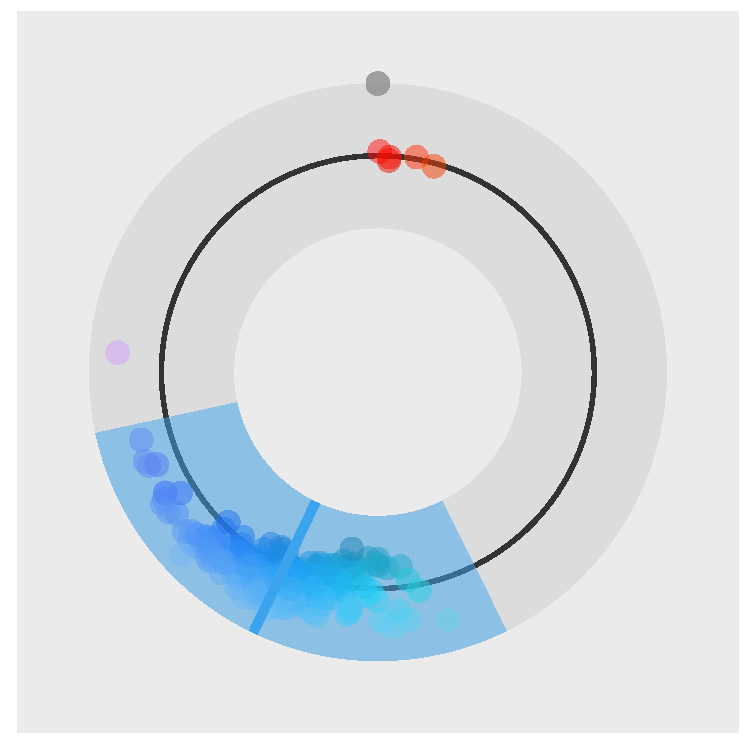
\includegraphics[width=\linewidth]{single_column.pdf}
	\caption{\textbf{A random visualization.} This is an example of a figure that spans only across one of the two columns.}
	\label{fig:column}
\end{figure}

On the other hand, \figurename~\ref{fig:whole} is an example of a figure that spans across the whole page (across both columns) of the report.

% \begin{figure*} makes the figure take up the entire width of the page
\begin{figure*}[ht]\centering 
	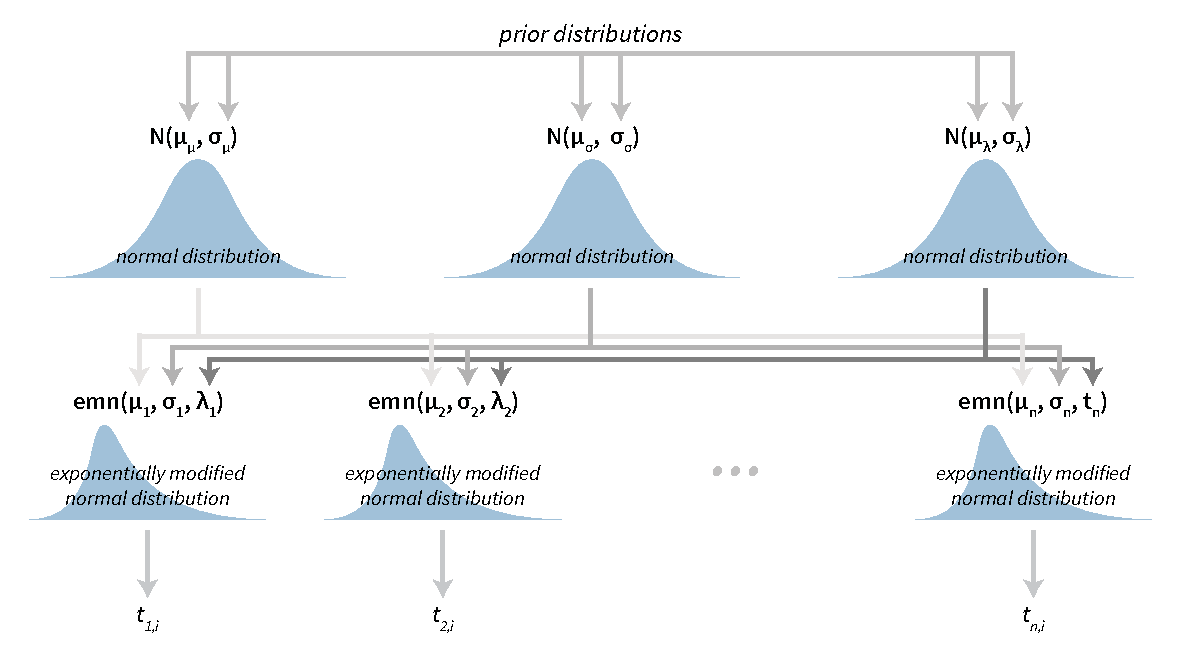
\includegraphics[width=\linewidth]{whole_page.pdf}
	\caption{\textbf{Visualization of a Bayesian hierarchical model.} This is an example of a figure that spans the whole width of the report.}
	\label{fig:whole}
\end{figure*}


\subsection*{Tables}

Use the table environment to insert tables.

\begin{table}[hbt]
	\caption{Table of grades.}
	\centering
	\begin{tabular}{l l | r}
		\toprule
		\multicolumn{2}{c}{Name} \\
		\cmidrule(r){1-2}
		First name & Last Name & Grade \\
		\midrule
		John & Doe & $7.5$ \\
		Jane & Doe & $10$ \\
		Mike & Smith & $8$ \\
		\bottomrule
	\end{tabular}
	\label{tab:label}
\end{table}


\subsection*{Code examples}

You can also insert short code examples. You can specify them manually, or insert a whole file with code. Please avoid inserting long code snippets, advisors will have access to your repositories and can take a look at your code there. If necessary, you can use this technique to insert code (or pseudo code) of short algorithms that are crucial for the understanding of the manuscript.

\lstset{language=Python}
\lstset{caption={Insert code directly from a file.}}
\lstset{label={lst:code_file}}
\lstinputlisting[language=Python]{code/example.py}

\lstset{language=R}
\lstset{caption={Write the code you want to insert.}}
\lstset{label={lst:code_direct}}
\begin{lstlisting}
import(dplyr)
import(ggplot)

ggplot(diamonds,
	   aes(x=carat, y=price, color=cut)) +
  geom_point() +
  geom_smooth()
\end{lstlisting}

%------------------------------------------------

\section*{Results}

The initial results of the fine-tuned model are promising. When context from the validation set is inserted into the model, it produces questions in Slovene, whereas before fine-tuning they were a mixture of languages and alphabets, mainly Russian. The questions do cover the topic in the context, but they tend to focus on some very specific aspects of the context or give questions that are grammatically a bit lacking. This might be the result of the Slovenian SQuAD translation having similar grammatical errors. When the model is fed passages from the Slovenian wikipedia, it provides questions that make sense and are true to the topic.


TODO: manual check of a large amount of questions, framework for evaluation.


Use the results section to present the final results of your work. Present the results in a objective and scientific fashion. Use visualisations to convey your results in a clear and efficient manner. When comparing results between various techniques use appropriate statistical methodology.

\subsection*{More random text}

This text is inserted only to make this template look more like a proper report. Lorem ipsum dolor sit amet, consectetur adipiscing elit. Etiam blandit dictum facilisis. Lorem ipsum dolor sit amet, consectetur adipiscing elit. Interdum et malesuada fames ac ante ipsum primis in faucibus. Etiam convallis tellus velit, quis ornare ipsum aliquam id. Maecenas tempus mauris sit amet libero elementum eleifend. Nulla nunc orci, consectetur non consequat ac, consequat non nisl. Aenean vitae dui nec ex fringilla malesuada. Proin elit libero, faucibus eget neque quis, condimentum laoreet urna. Etiam at nunc quis felis pulvinar dignissim. Phasellus turpis turpis, vestibulum eget imperdiet in, molestie eget neque. Curabitur quis ante sed nunc varius dictum non quis nisl. Donec nec lobortis velit. Ut cursus, libero efficitur dictum imperdiet, odio mi fermentum dui, id vulputate metus velit sit amet risus. Nulla vel volutpat elit. Mauris ex erat, pulvinar ac accumsan sit amet, ultrices sit amet turpis.

Phasellus in ligula nunc. Vivamus sem lorem, malesuada sed pretium quis, varius convallis lectus. Quisque in risus nec lectus lobortis gravida non a sem. Quisque et vestibulum sem, vel mollis dolor. Nullam ante ex, scelerisque ac efficitur vel, rhoncus quis lectus. Pellentesque scelerisque efficitur purus in faucibus. Maecenas vestibulum vulputate nisl sed vestibulum. Nullam varius turpis in hendrerit posuere.

Nulla rhoncus tortor eget ipsum commodo lacinia sit amet eu urna. Cras maximus leo mauris, ac congue eros sollicitudin ac. Integer vel erat varius, scelerisque orci eu, tristique purus. Proin id leo quis ante pharetra suscipit et non magna. Morbi in volutpat erat. Vivamus sit amet libero eu lacus pulvinar pharetra sed at felis. Vivamus non nibh a orci viverra rhoncus sit amet ullamcorper sem. Ut nec tempor dui. Aliquam convallis vitae nisi ac volutpat. Nam accumsan, erat eget faucibus commodo, ligula dui cursus nisi, at laoreet odio augue id eros. Curabitur quis tellus eget nunc ornare auctor.


%------------------------------------------------

\section*{Discussion}

Use the Discussion section to objectively evaluate your work, do not just put praise on everything you did, be critical and exposes flaws and weaknesses of your solution. You can also explain what you would do differently if you would be able to start again and what upgrades could be done on the project in the future.


%------------------------------------------------

\section*{Acknowledgments}

Here you can thank other persons (advisors, colleagues ...) that contributed to the successful completion of your project.


%----------------------------------------------------------------------------------------
%	REFERENCE LIST
%----------------------------------------------------------------------------------------
\bibliographystyle{unsrt}
\bibliography{report}


\end{document}